%
% ground_segment.tex
%
% Copyright (C) 2021 by SpaceLab.
%
% GOLDS-UFSC Documentation
%
% This work is licensed under the Creative Commons Attribution-ShareAlike 4.0
% International License. To view a copy of this license,
% visit http://creativecommons.org/licenses/by-sa/4.0/.
%

%
% \brief Ground segment chapter.
%
% \author Gabriel Mariano Marcelino <gabriel.mm8@gmail.com>
%
% \institution Universidade Federal de Santa Catarina (UFSC)
%
% \version 0.1.0
%
% \date 2020/06/06
%

\chapter{Ground Segment} \label{ch:ground-segment}

\section{Hardware}

.

\section{Satellite Tracking}

To track the satellite and for orbit prediction, the GPredict software \cite{gpredict} will be used.

A picture of the main window of GPredict can be seen in \autoref{fig:gpredict}.

\begin{figure}[!ht]
    \begin{center}
        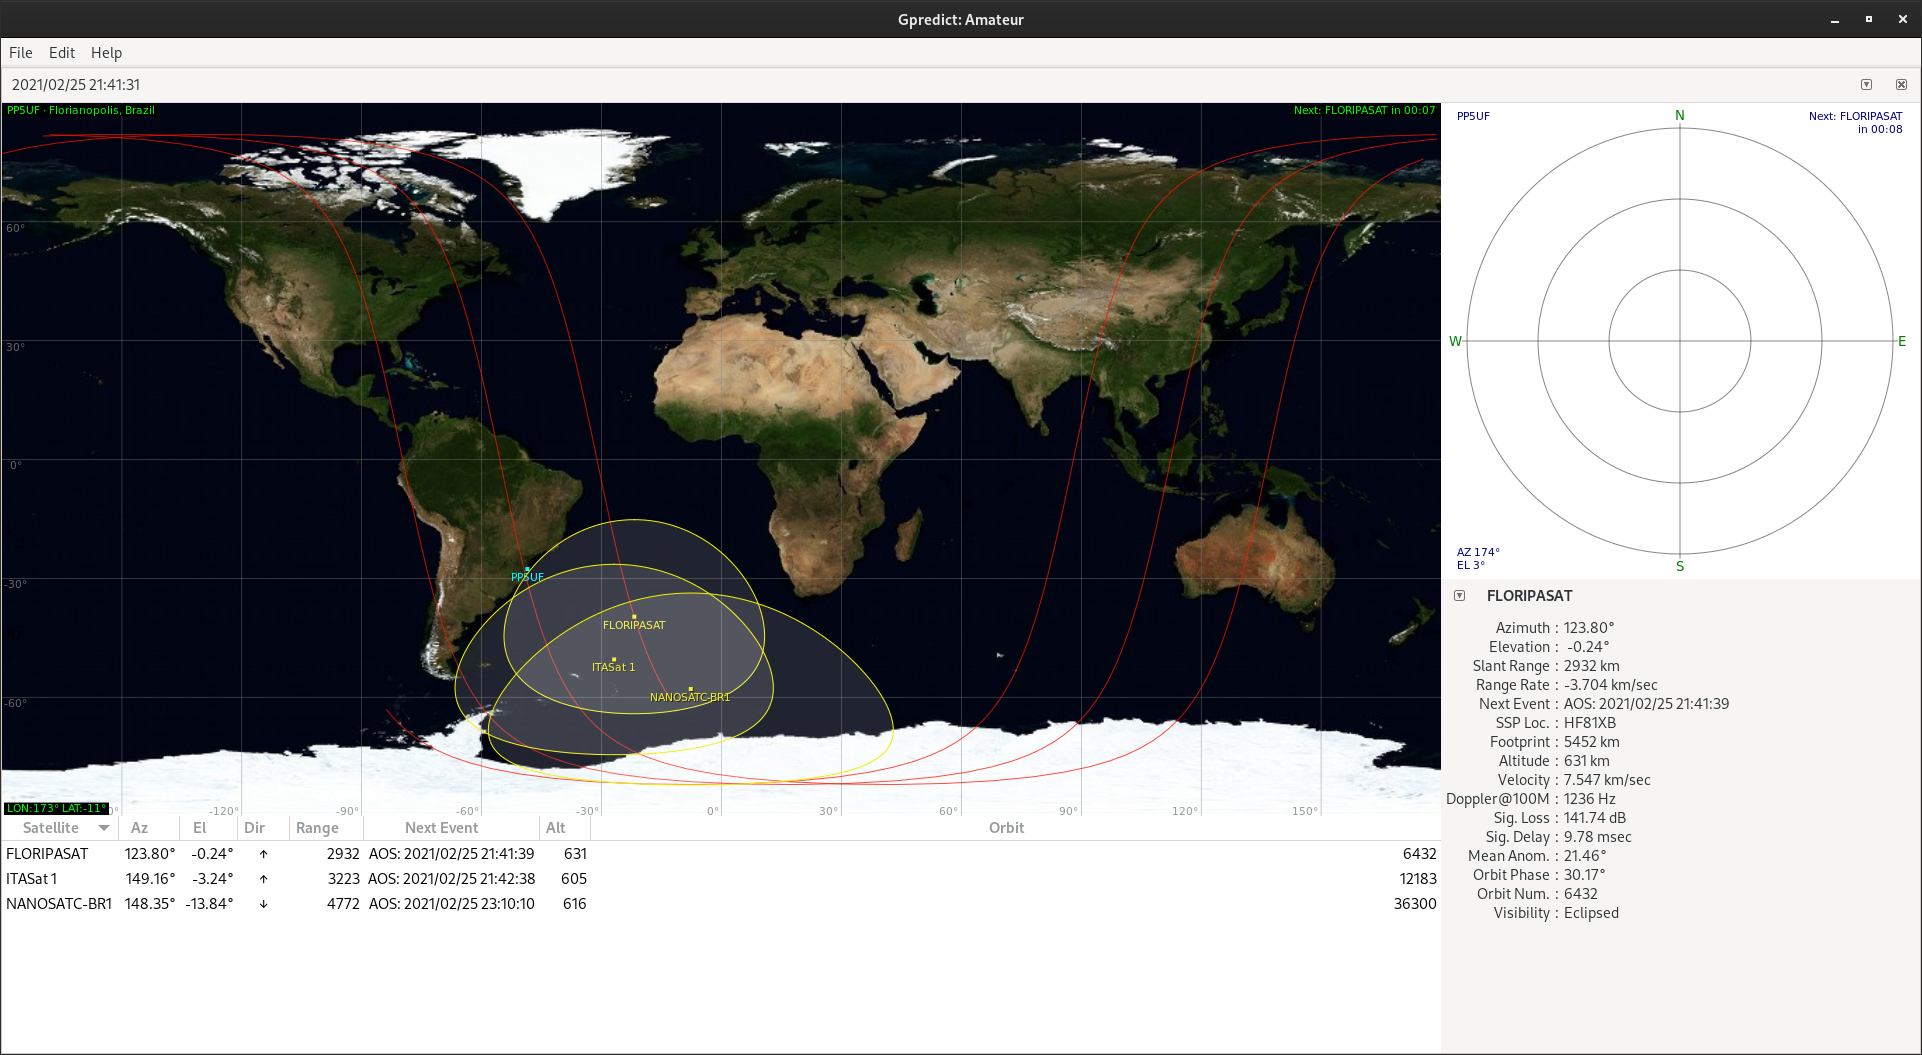
\includegraphics[width=\textwidth]{figures/gpredict.png}
        \caption{Main window of GPredict.}
        \label{fig:gpredict}
    \end{center}
\end{figure}
